\RequirePackage[l2tabu,orthodox]{nag}  % warn about common LaTeX pitfalls
\RequirePackage[ascii]{inputenc}  % input is 7-bit ASCII
\RequirePackage{fixltx2e}  % fix LaTeX2e kernel bugs

\documentclass[11pt,twoside]{article}
\usepackage{color}
\usepackage{graphicx}
\graphicspath{ {image/} }
\usepackage{calc}  % arithmetic in length parameters
\usepackage{enumitem}  % more control over list formatting
\usepackage{fancyhdr}  % simpler headers and footers
\usepackage[margin=1in]{geometry}  % page layout
\usepackage{lastpage}  % for last page number
\usepackage{relsize}  % easier font size changes
\usepackage[normalem]{ulem}  % smarter underlining
\usepackage{url}  % verb-like typesetting of URLs
\usepackage{xfrac}  % nicer looking simple fractions for text and math
\usepackage{longtable}
\usepackage{tikz}
\usepackage{array}
\usepackage{tikz-timing}
\usetikzlibrary{arrows, shapes, backgrounds,fit}
\usepackage{tkz-graph}
% Set up fonts.
\usepackage[T1]{fontenc}  % use true 8-bit fonts
\usepackage{slantsc}  % allow slanted small-caps
\usepackage{microtype}  % perform various font optimizations
% Use Palatino-based monospace instead of kpfonts' default.
%\usepackage{newpxtext}
\ttfamily
\DeclareFontShape{T1}{\ttdefault}{m}{scsl}{<->ssub*\ttdefault/m/sc}{}
\DeclareFontShape{T1}{\ttdefault}{b}{scsl}{<->ssub*\ttdefault/b/sc}{}
% "Kepler" fonts.
\usepackage[nott,notextcomp]{kpfonts}
% Use curvier Latin Modern brackets instead of kpfonts' glyphs.
\DeclareSymbolFont{lmsymb}     {OMS}{lmsy}{m}{n}
\DeclareSymbolFont{lmlargesymb}{OMX}{lmex}{m}{n}
\DeclareMathDelimiter{\rbrace}{\mathclose}{lmsymb}{"67}{lmlargesymb}{"09}
\DeclareMathDelimiter{\lbrace}{\mathopen}{lmsymb}{"66}{lmlargesymb}{"08}

% Page layout: stretch text to fill up page.
\addtolength\footskip{.25\headheight}
\flushbottom

% Common list settings.

% Common macros.
%%  Common macros for the course CSC263H1 at the University of Toronto.
%%
%%  Copyright (c) 2014 Francois Pitt <fpitt@cs.utoronto.ca>
%%  last updated at 17:53 (EDT) on Sun 19 Oct 2014
%%
%%  CC BY-SA 4.0
%%  This work (the current file named 'macros-263.tex') is licensed under
%%  the Creative Commons Attribution-ShareAlike 4.0 International License.
%%  To view a copy of this license, visit
%%      http://creativecommons.org/licenses/by-sa/4.0/
%%  or send a letter to: Creative Commons, 444 Castro Street, Suite 900,
%%  Mountain View, California, 94041, USA.
%%  This is a human-readable summary of (and not a substitute for) the
%%  license.
%%  You are free to:
%%      Share -- copy and redistribute the material in any medium or format
%%      Adapt -- remix, transform, and build upon the material for any
%%          purpose, even commercially.
%%      The licensor cannot revoke these freedoms as long as you follow the
%%          license terms.
%%  Under the following terms:
%%      Attribution -- You must give appropriate credit, provide a link to
%%          the license, and indicate if changes were made. You may do so in
%%          any reasonable manner, but not in any way that suggests the
%%          licensor endorses you or your use.
%%      ShareAlike -- If you remix, transform, or build upon the material,
%%          you must distribute your contributions under the same license as
%%          the original.
%%      No additional restrictions -- You may not apply legal terms or
%%          technological measures that legally restrict others from doing
%%          anything the license permits.
%%  Notices:
%%      You do not have to comply with the license for elements of the
%%      material in the public domain or where your use is permitted by an
%%      applicable exception or limitation.
%%      No warranties are given. The license may not give you all of the
%%      permissions necessary for your intended use. For example, other
%%      rights such as publicity, privacy, or moral rights may limit how you
%%      use the material.

% Redefine \today in the style "DD Month YYYY".
\renewcommand*\today
 {\number\day\space\ifcase\month\or January\or February\or March\or
  April\or May\or June\or July\or August\or September\or October\or
  November\or December\fi\space\number\year}

% TeX trick so that math symbols are bold when text is.
\let\seiresfb\bfseries\def\bfseries{\boldmath\seiresfb}
\let\seiresdm\mdseries\def\mdseries{\unboldmath\seiresdm}

% Centered version of \llap and \rlap.
\providecommand*\clap[1]{\hbox to 0pt{\hss#1\hss}}

% Spacing macros with default argument.
\providecommand*\vfillstretch[1][1]{\vspace*{\stretch{#1}}}
\providecommand*\hfillstretch[1][1]{\hspace*{\stretch{#1}}}

% Abbreviations of latin phrases.
\let\latinabb\empty  % no special formatting
\providecommand*\ie{\latinabb{i.e.}}
\providecommand*\eg{\latinabb{e.g.}}
\providecommand*\etc{\latinabb{etc}}
\providecommand*\vs{\latinabb{vs}}

% General fonts and characters.
\let\longemph\textsl  % alternate way to emphasize
\let\strong\textbf  % strong emphasis
\let\code\texttt  % code fragments
\let\var\textsl  % multi-letter variables
\let\pred\mathbf  % predicates
\providecommand*\stup{\textsuperscript{st}}
\providecommand*\ndup{\textsuperscript{nd}}
\providecommand*\rdup{\textsuperscript{rd}}
\providecommand*\thup{\textsuperscript{th}}
\newcommand*\bbmath[1]{\ensuremath{\mathbb{#1}}}  % requires amssymb
\providecommand*\N{\bbmath{N}}  % requires amssymb
\providecommand*\Z{\bbmath{Z}}  % requires amssymb
\providecommand*\Q{\bbmath{Q}}  % requires amssymb
\providecommand*\R{\bbmath{R}}  % requires amssymb
\providecommand*\bigOh{\mathcal{O}}
\providecommand*\onehalf{\ensuremath{{}^1\!\!/\!_2}}
\providecommand*\letlinebreak{\penalty\exhyphenpenalty}
\providecommand*\halfthinspace{\kern.083333em}
\providecommand*\dash
   {\letlinebreak\halfthinspace---\halfthinspace\letlinebreak}
\let\per\slash  % for convenience

% For defined terms -- requires package ulem.
\newcommand*\defn[1]{\uline{\textit{#1}}}
\setlength{\ULdepth}{.2ex}

% General math macros.
\newcommand*\hiderel[1]{\mathrel{\hphantom{#1}}}
\providecommand*\comp[1]{\overline{#1}}  % set complement
\providecommand*\emptystr{\varepsilon}  % empty string
\providecommand*\lxor{\mathbin\oplus}  % exclusive or
\providecommand*\cat{\cdot}  % string concatenation
% Floors and ceilings, with optional size-changing command, e.g.,
% \floor[\Big]{x/2} becomes '\Big\lfloor{x/2}\Big\rfloor'.
\providecommand*\floor[2][]{{#1\lfloor}{#2}{#1\rfloor}}
\providecommand*\ceil[2][]{{#1\lceil}{#2}{#1\rceil}}
\providecommand*\lcm{\operatorname{lcm}}  % requires amsmath
\providecommand*\size{\operatorname{size}}  % requires amsmath
\providecommand*\len{\operatorname{len}}  % requires amsmath
\providecommand*\divides{\mathrel{|}}

% Redefined symbols from amssymb.
\renewcommand*\emptyset{\varnothing}  % rounder than default
\let\bigiff\iff
\renewcommand*\iff{\mathrel{\Leftrightarrow}}  % smaller than default
\let\bigimplies\implies
\renewcommand*\implies{\mathrel{\Rightarrow}}  % smaller than default
\renewcommand*\ge{\geqslant}  % with slanted line under the > sign
\renewcommand*\le{\leqslant}  % with slanted line under the < sign

% For algorithms, using either CLRS-style or Python-style pseudocode.
\let\ADT\textsc  % ADT names
\let\proc\textsc  % function names
\let\const\textsc  % constants (True, False, etc.)
\let\kw\textbf  % keywords (if, while, etc.)
\providecommand*\comm[1]{\textsl{\#\space#1}}  % comments
\providecommand*\opgets[1]{\mathrel{#1=}}
\providecommand*\eq{\mathrel{==}}
\providecommand*\True{\const{True}}
\providecommand*\False{\const{False}}
\providecommand*\None{\const{None}}
\providecommand*\cmod{\mathbin{\%}}
\providecommand*\nil{\const{nil}}

% Checkboxes and checklists.
% \checkmark already defined in amssymb
\makeatletter
\@ifpackageloaded{kpfonts}
   {\newcommand*\exmark{$\times$}}
   {\newcommand*\exmark{{\boldmath$\times$}}}
\makeatother
\newlength\exmarksize
\newlength\exmarkdepth
\newcommand*\checkbox[1][]
   {\settoheight\exmarksize{\exmark}
    \settodepth\exmarkdepth{\exmark}
    \addtolength\exmarksize{-\exmarkdepth}
    {\setlength\fboxrule{.1ex}\setlength\fboxsep{.1ex}%
    \fbox{\rule{0pt}{\exmarksize}\makebox[\exmarksize]{\smash{#1}}}}}
\newcommand*\checkedbox{\checkbox[\raisebox{.1ex}{\kern.2em$\checkmark$}]}
\newcommand*\exedbox{\checkbox[\exmark]}
\newenvironment*{checklist}{\begin{list}{\checkbox}{}}{\end{list}}
\newcommand*\checkeditem{\item[\checkedbox]}
\newcommand*\exeditem{\item[\exedbox]}
\newcommand*\boxeditem[1][]{\item[{\checkbox[#1]}]}

% Macros for drawing "underline" rules and half-boxes.
\providecommand*\urule[2][.5pt]{\rule[-.4ex]{#2}{#1}} % "underline" rule
% Underlined text box (with optional positioning argument).
\providecommand*\ubox[3][c]{\rlap{\urule{#2}}\makebox[#2][#1]{#3}}
% Underlined text box with caption (and optional caption positioning).
\providecommand*\capbox[5][c]{\ifx\empty#2\empty
    \else\rlap{\raisebox{-\baselineskip}{\makebox[#3][#1]{#2}}}\fi
    \ubox[#4]{#3}{#5}}

% For student numbers.
\providecommand*\hb{\urule{1.2em}}      % horizontal bar
\providecommand*\vb{\urule[1ex]{.5pt}}  % vertical bar
\providecommand*\studentnumberboxes     % now 10-digits long!
   {\vb\hb\vb\hb\vb\hb\vb\hb\vb\hb\vb\hb\vb\hb\vb\hb\vb\hb\vb\hb\vb}
\newlength\numberboxwidth
\settowidth\numberboxwidth{\studentnumberboxes}

% Command to format sample solutions for tutorials.
\newcommand\samplesolution[1]
   {\ifsolutions\begin{quote}\sffamily{#1}\end{quote}\fi}

% Marking-related macros.
\providecommand*\markitem[2][]
   {\item{\bfseries#2}\ifx\empty#1\empty\else
    \space[$#1$ mark\ifnum#1>1 s\fi]\fi:\quad\ignorespaces}
\providecommand*\errorcode[2][]
   {\item{\bfseries error code #2}\ifx\empty#1\empty\else
    \space[#1]\fi:\quad\ignorespaces}
\providecommand*\commonerror[1][]
   {\item{\bfseries common error}\ifx\empty#1\empty\else
    \space[#1]\fi:\quad\ignorespaces}
\makeatletter
\providecommand*\heading[1]%
   {\@startsection{heading}{9}{0pt}{-.75ex plus -1.5ex minus -.5ex}
    {-.5em plus -.5em minus -.25em}{\normalfont}*{\textsc{#1}}\mbox{}}
\makeatother
\newcommand*\st{\mathrel{|}}  % "such that" for set extension

% Headings.
\pagestyle{fancy}
\let\headrule\empty
\let\footrule\empty
\lhead{CSC\,336\,H1}
\chead{\large\scshape Assignment \#\,3}
\rhead{\scshape Fall 2015}
\lfoot{\scshape Dept.\@ of Computer Science, University of Toronto,
       St.~George Campus}
\cfoot{}
\rfoot{\scshape page \thepage\space of \pageref{LastPage}}


\begin{document}

\begin{enumerate}[leftmargin=0pt]
% question 1
\item
	\begin{enumerate}
	% part a
	\item  
	\[|g_1'(x)| = |\frac{2x}{3}| \Rightarrow |g_1'(2)| = \frac{4}{3} > 1 \]
	\[|g_2'(x)| = |\frac{3}{2 \sqrt{3x-2}}|  \Rightarrow |g_2'(2)| = \frac{3}{4} < 1\]
	\[|g_3'(x)| = |\frac{2}{x^2}|  \Rightarrow |g_3'(2)| = \frac{1}{2} < 1\]
	\[|g_4'(x)| = |\frac{2x(2x-3) - 2(x^2-2)}{(2x-3)^2}| \Rightarrow |g_4'(2)| = \frac{4-4}{1} = 0\]
	Then we know that $ |g_1'(2)|$  is bigger than 1, which means divergence. $|g_2'(2) = \frac{3}{4}|$ means it is 
	linear convergence with constant  $|\frac{3}{4}|$.   $|g_3'(2) = \frac{1}{2}|$ means it is linear convergence with constant  $|\frac{1}{2}|$. And  $|g_4'(2) = 0|$ means it is quadratic convergence.
 	%part b
	\item
	\[ 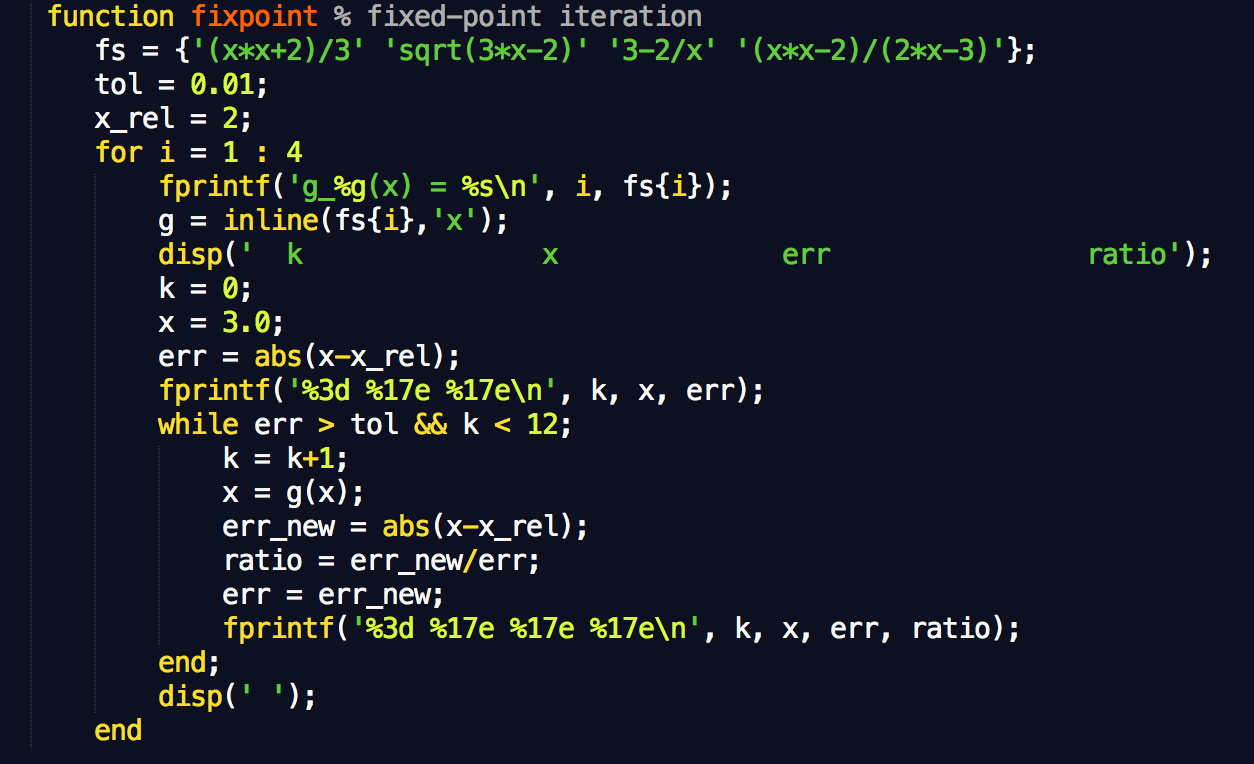
\includegraphics[scale=0.5]{1b} \]
	\[ 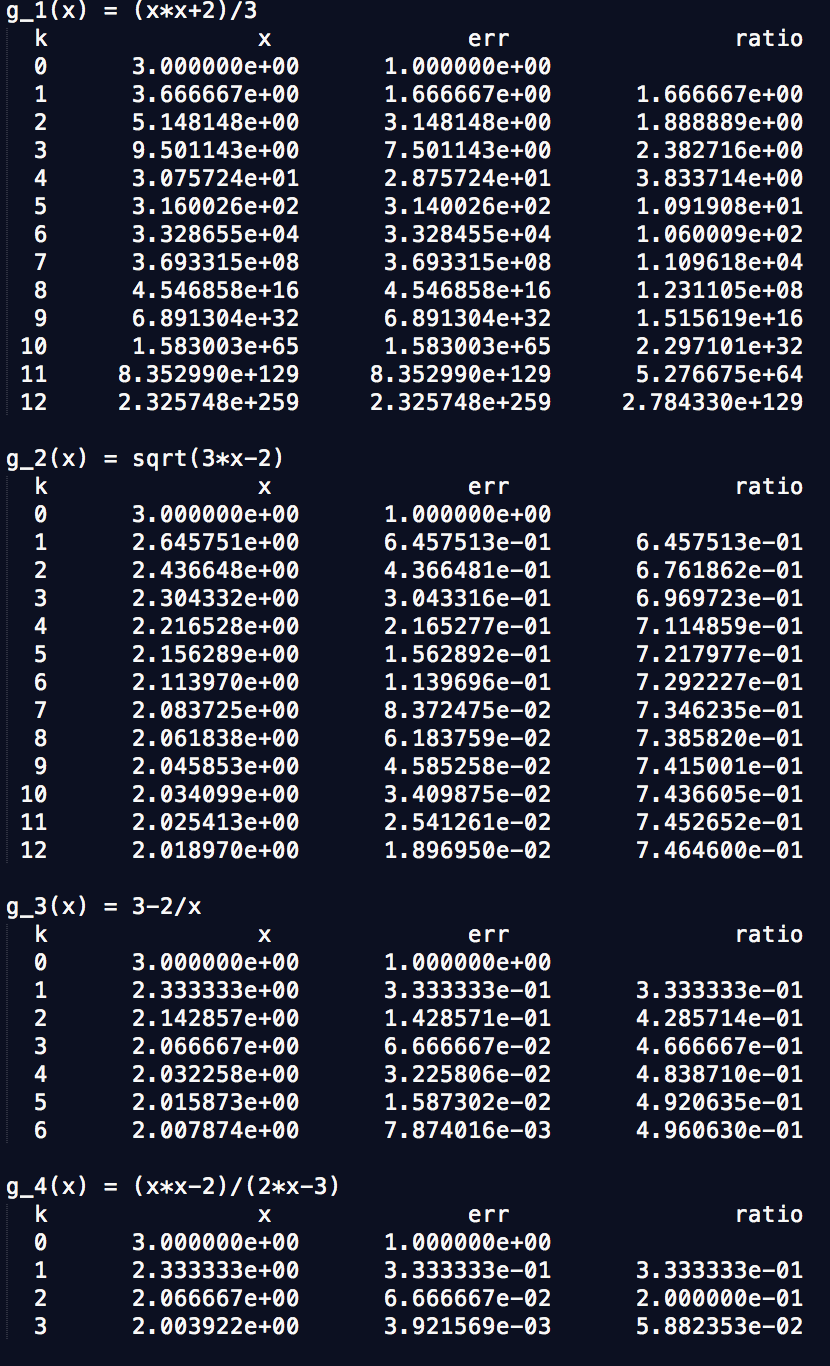
\includegraphics[scale=0.5]{1br} \]
	Clearly, the converging rate is approximately like what we calculated. 
	\end{enumerate}
% question 2
\item
	\begin{enumerate}
	\item Starting with the secant method update formula is given as
				\[x_{k+1} = x_k - \frac{f(x_k)(x_k-x_{k-1})}{f(x_k)-f(x_{k-1})}\]
				\[=  \frac{x_k(f(x_k)-f(x_{k-1})) - f(x_k)(x_k-x_{k-1})}{f(x_k)-f(x_{k-1})}\]
				\[=  \frac{x_k f(x_k) - x_k f(x_{k-1}) - x_kf(x_k)+x_{k-1}f(x_k)}{f(x_k)-f(x_{k-1})}\]
				\[=  \frac{x_{k-1} f(x_k) - x_k f(x_{k-1})} {f(x_k)-f(x_{k-1})}\]
	\item  When we close to solution then $x_{k-1}$ and $x_k$ are close to each other which mean there difference is close to $0$, and also can cause  catastrophic cancellation. For formula in $part (a) $ it is hard for us to get rid of cancellation. For formula in $part (b)$, catastrophic cancellation is the only thing affecting $x_{k+1}$

	\end{enumerate}

% question 3
\item
	\[ 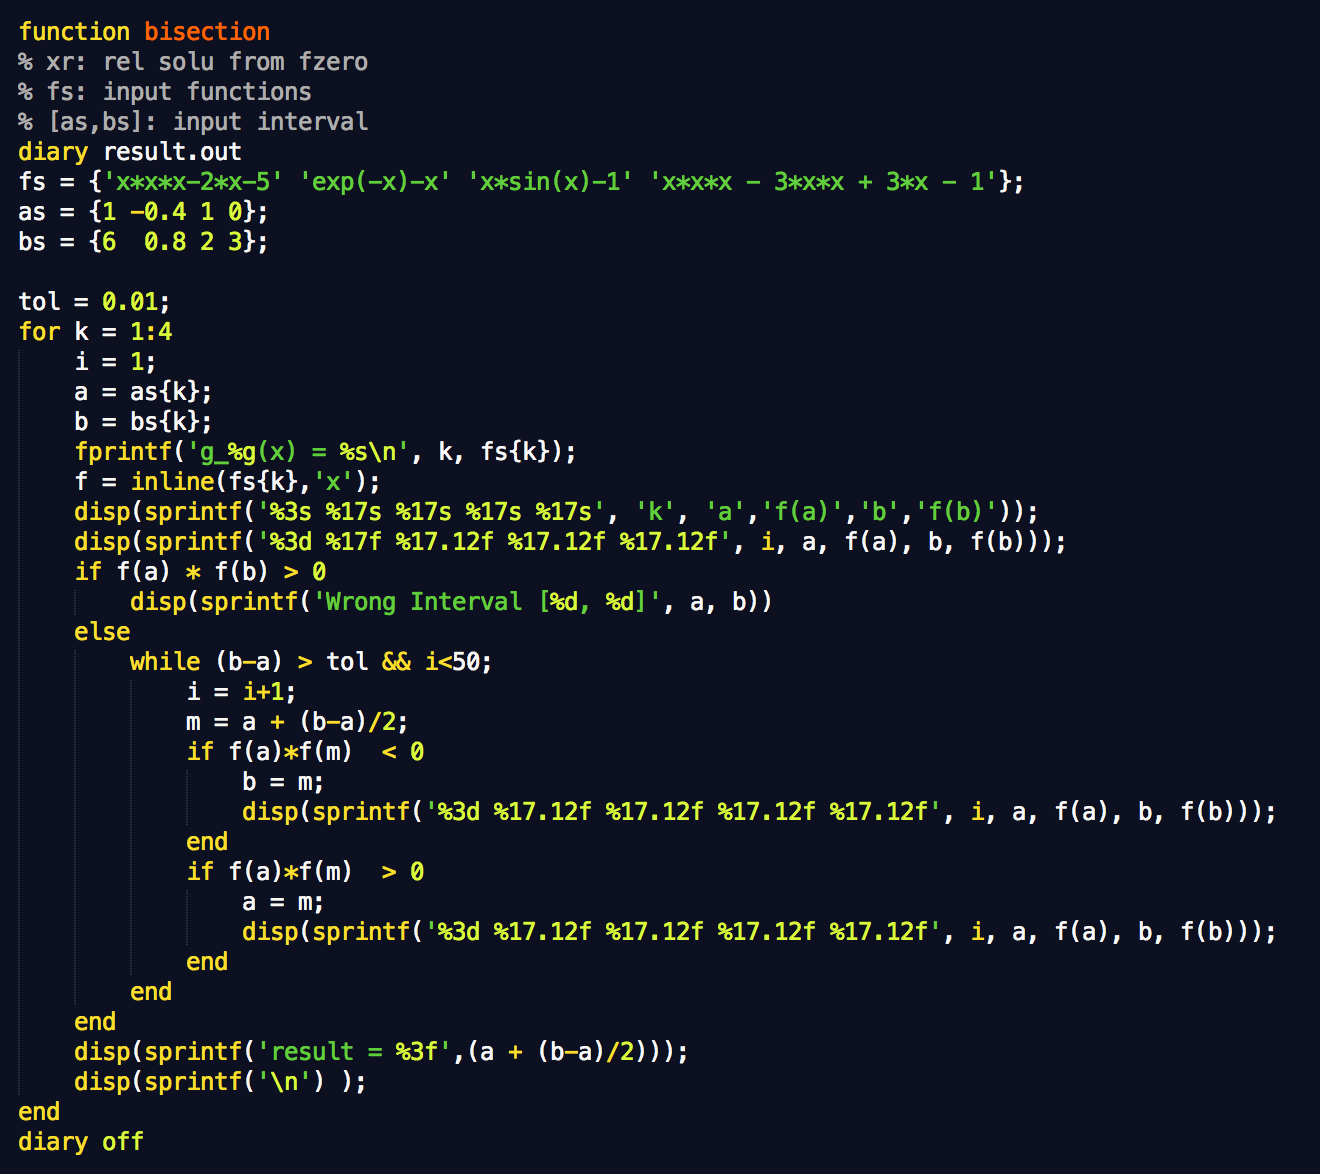
\includegraphics[scale=0.35]{3b} \]
	\[ 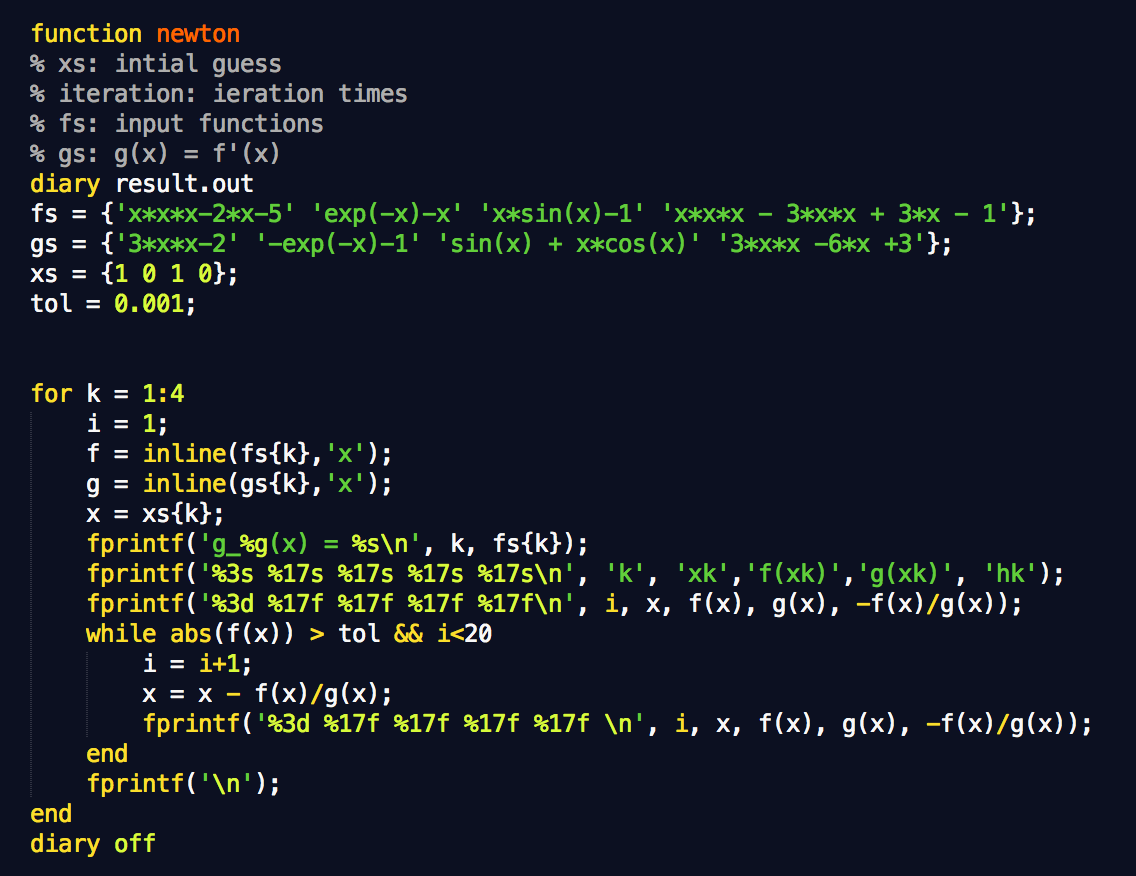
\includegraphics[scale=0.35]{3n} \]
	\[ 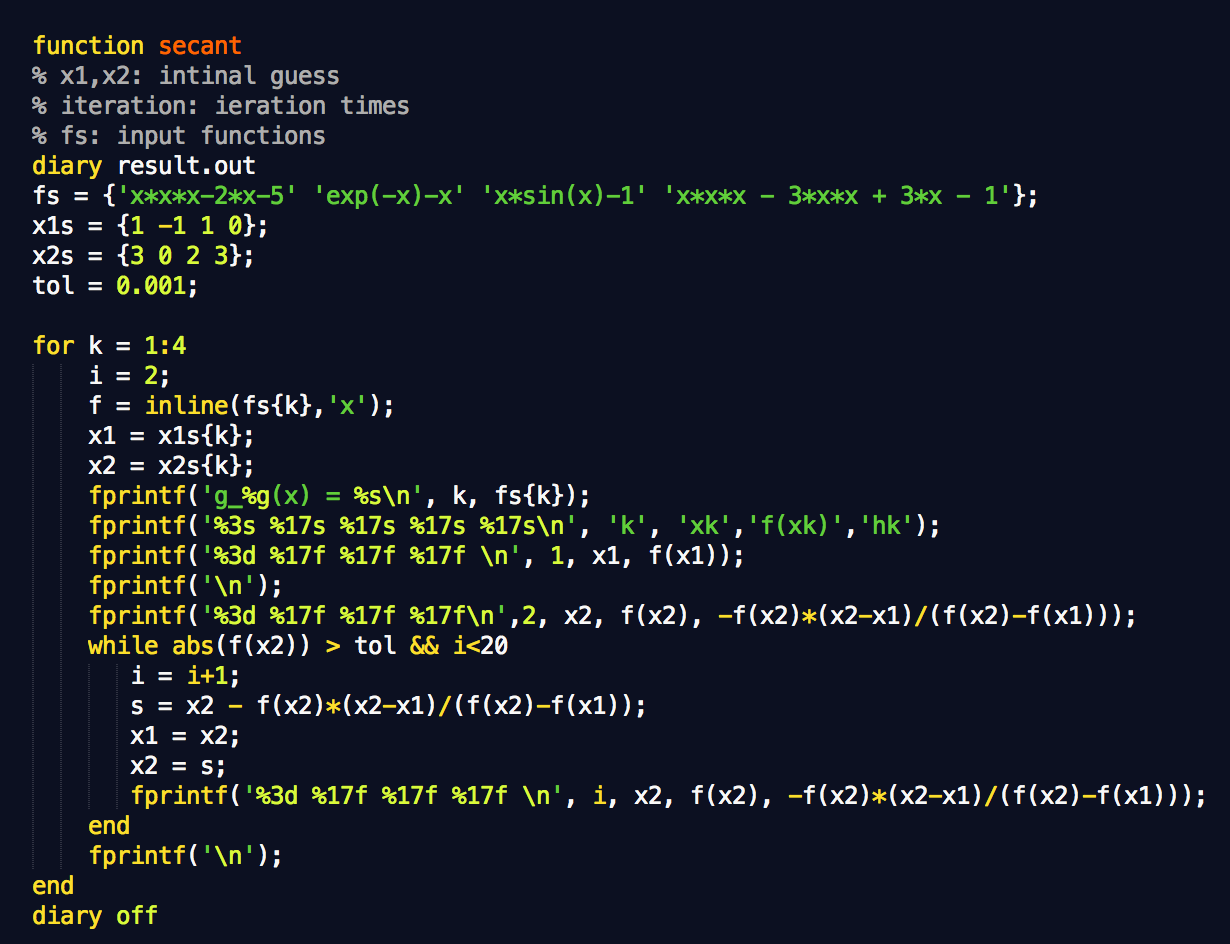
\includegraphics[scale=0.35]{3s} \]
	For termination criteria, 
	\begin{itemize}[label = {}]
		\item using $b-a > tol$ for bisection;
		\item using $f(x) > tol $ for Newton's method;
		\item using $f(x) > tol $ for secant.
	\end{itemize}
	\begin{enumerate}
	% part a
	\item 	\[f(x): x^3 - 2x - 5 = 0\]
		  	\[f'(x): 3x^2 -2\]
		% bisection
		$bisection: $
		 \begin{longtable}{|>{\tiny}p{0.5in}|>{\tiny} p{0.5in}| >{\tiny}p{0.5in}|>{\tiny}p{0.5in}|	
		 	>{\tiny} p{0.8in}|}\hline
			iteration&interval&tolerance&root&convergence \ rate \\[0.1in]\hline
			12 &[1,3]&0.001&2.0947&linear around(0.5)\\[0.1in] \hline
		\end{longtable} 
		%newton
		$Newton's method:$
		 \begin{longtable}{|>{\tiny}p{0.5in}|>{\tiny} p{0.5in}| >{\tiny}p{0.5in}|>{\tiny}p{0.5in}|	
		 	>{\tiny} p{0.8in}|}\hline
			iteration&initial \ guess&tolerance&root&convergence \ rate \\[0.1in]\hline
			8 &1&0.001&2.0946&linear around $10^{-1}$\\[0.1in] \hline
		\end{longtable} 
		%secant
		$secant:$
		\begin{longtable}{|>{\tiny}p{0.5in}|>{\tiny} p{0.5in}| >{\tiny}p{0.5in}|>{\tiny}p{0.5in}|	
		 	>{\tiny} p{0.8in}|}\hline
			iteration&initial \ guess&tolerance&root&convergence \ rate \\[0.1in]\hline
			8 &1,3&0.001&2.0946& linear($10^{-1}$)\\[0.1in] \hline
		\end{longtable} 
		$fzero:$ \\
		Using matlab  $fzero$ with initial guess $1$, we get a root $2.0946$.

	% part b
	\item 	\[ e^{-x} = x\]
			\[-e^{-x} = 1\]
		% bisection
		$bisection: $
		 \begin{longtable}{|>{\tiny}p{0.5in}|>{\tiny} p{0.5in}| >{\tiny}p{0.5in}|>{\tiny}p{0.5in}|	
		 	>{\tiny} p{0.8in}|}\hline
			iteration&interval&tolerance&root&convergence \ rate \\[0.1in]\hline
			11 &[0,1]&0.001&0.5674&linear around(0.5)\\[0.1in] \hline
		\end{longtable} 
		%newton
		$Newton's method:$
		 \begin{longtable}{|>{\tiny}p{0.5in}|>{\tiny} p{0.5in}| >{\tiny}p{0.5in}|>{\tiny}p{0.5in}|	
		 	>{\tiny} p{0.8in}|}\hline
			iteration&initial \ guess&tolerance&root&convergence \ rate \\[0.1in]\hline
			4 &0&0.001&0.5671&linear($10^{-1}$)\\[0.1in] \hline
		\end{longtable} 
		%secant
		$secant:$
		\begin{longtable}{|>{\tiny}p{0.5in}|>{\tiny} p{0.5in}| >{\tiny}p{0.5in}|>{\tiny}p{0.5in}|	
		 	>{\tiny} p{0.8in}|}\hline
			iteration&initial \ guess&tolerance&root&convergence \ rate \\[0.1in]\hline
			5 &0,1&0.001&0.5672& linear($10^{-1}$)\\[0.1in] \hline
		\end{longtable} 
		$fzero:$ \\
		Using matlab  $fzero$ with initial guess $1$, we get a root $0.5671$.

	%part c
	\item \[x\sin(x) = 1\]
		 \[\sin(x) + x\cos(x) = 0\]
		% bisection
		$bisection: $
		 \begin{longtable}{|>{\tiny}p{0.5in}|>{\tiny} p{0.5in}| >{\tiny}p{0.5in}|>{\tiny}p{0.5in}|	
		 	>{\tiny} p{0.8in}|}\hline
			iteration&interval&tolerance&root&convergence \ rate \\[0.1in]\hline
			11 &[1,2]&0.001&1.1143&linear around(0.5)\\[0.1in] \hline
		\end{longtable} 
		%newton
		$Newton's method:$
		 \begin{longtable}{|>{\tiny}p{0.5in}|>{\tiny} p{0.5in}| >{\tiny}p{0.5in}|>{\tiny}p{0.5in}|	
		 	>{\tiny} p{0.8in}|}\hline
			iteration&initial \ guess&tolerance&root&convergence \ rate \\[0.1in]\hline
			2 &0.5&0.001&1.1147&linear($10^{-1}$)\\[0.1in] \hline
		\end{longtable} 
		%secant
		$secant:$
		\begin{longtable}{|>{\tiny}p{0.5in}|>{\tiny} p{0.5in}| >{\tiny}p{0.5in}|>{\tiny}p{0.5in}|	
		 	>{\tiny} p{0.8in}|}\hline
			iteration&initial \ guess&tolerance&root&convergence \ rate \\[0.1in]\hline
			5 &1,2&0.001&1.1142&super linear (1.5)\\[0.1in] \hline
		\end{longtable} 
		$fzero:$ \\
		Using matlab  $fzero$ with initial guess $1$, we get a root $1.1142$.
	%part d
	\item \[x^3 -3x^2 +3x -1 = 0\]
		 \[3x^2 -6x + 3 = 0\]
		% bisection
		$bisection: $
		 \begin{longtable}{|>{\tiny}p{0.5in}|>{\tiny} p{0.5in}| >{\tiny}p{0.5in}|>{\tiny}p{0.5in}|	
		 	>{\tiny} p{0.8in}|}\hline
			iteration&interval&tolerance&root&convergence \ rate \\[0.1in]\hline
			12 &[0,3]&0.001&0.9998& linear(0.5)\\[0.1in] \hline
		\end{longtable} 
		%newton
		$Newton's method:$
		 \begin{longtable}{|>{\tiny}p{0.5in}|>{\tiny} p{0.5in}| >{\tiny}p{0.5in}|>{\tiny}p{0.5in}|	
		 	>{\tiny} p{0.8in}|}\hline
			iteration&initial \ guess&tolerance&root&convergence \ rate \\[0.1in]\hline
			7 &0&0.001&0.9122&linear(0.66)\\[0.1in] \hline
		\end{longtable} 
		%secant
		$secant:$
		\begin{longtable}{|>{\tiny}p{0.5in}|>{\tiny} p{0.5in}| >{\tiny}p{0.5in}|>{\tiny}p{0.5in}|	
		 	>{\tiny} p{0.8in}|}\hline
			iteration&initial \ guess&tolerance&root&convergence \ rate \\[0.1in]\hline
			11 &0,3&0.001&0.9232& linear(0.75)\\[0.1in] \hline
		\end{longtable} 
		$fzero:$ \\
		Using matlab  $fzero$ with initial guess $0$, we get a root $1.0000$.
	\end{enumerate}
% question 4
\item
	\begin{enumerate}
	% part a
	\item 
	\[ f(x) =\sqrt[3]{1-\frac{3}{4x}} = 0 \Rightarrow  1-\frac{3}{4x} = 0\]
	\[4x = 3 \Rightarrow x =\frac{3}{4}\]
	Hence, clearly function $ f(x) =\sqrt[3]{1-\frac{3}{4x}}$ only has one root which is $\frac{3}{4}$.
	%part b
	
	\item
	\[ 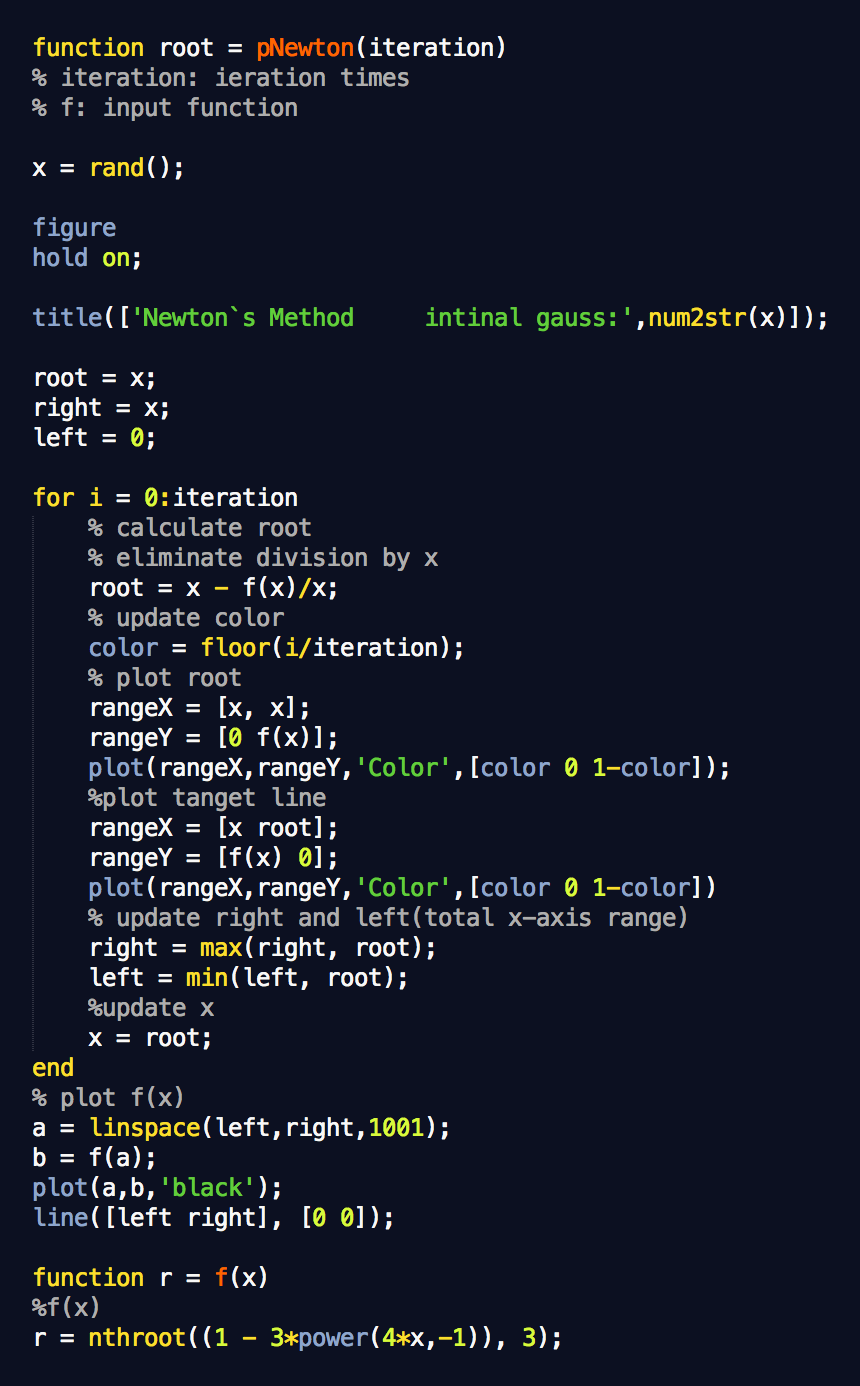
\includegraphics[scale=0.5]{4b} \]
	 5 plots of $Newton's \ method$ with random starting points show below, and the red line indicates the last iteration of the total 50 iterations.
		\[ 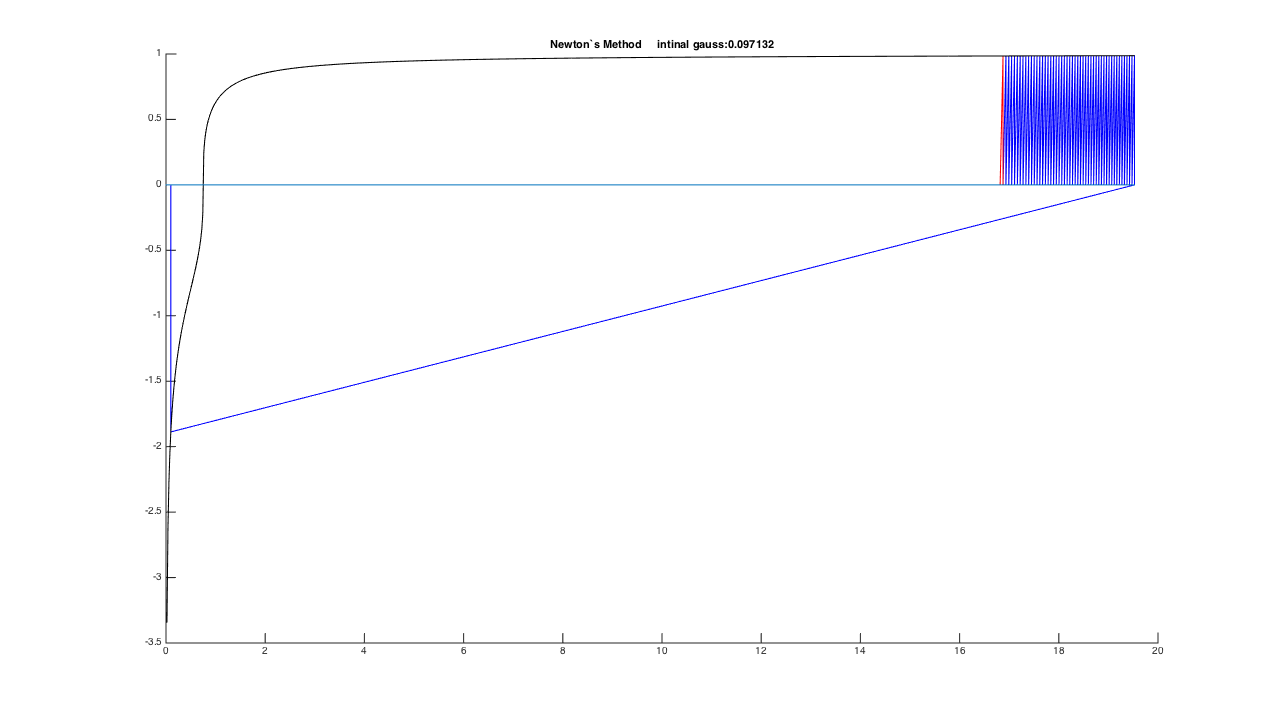
\includegraphics[scale=0.35]{plot(16-8175).png} \]
		\[ 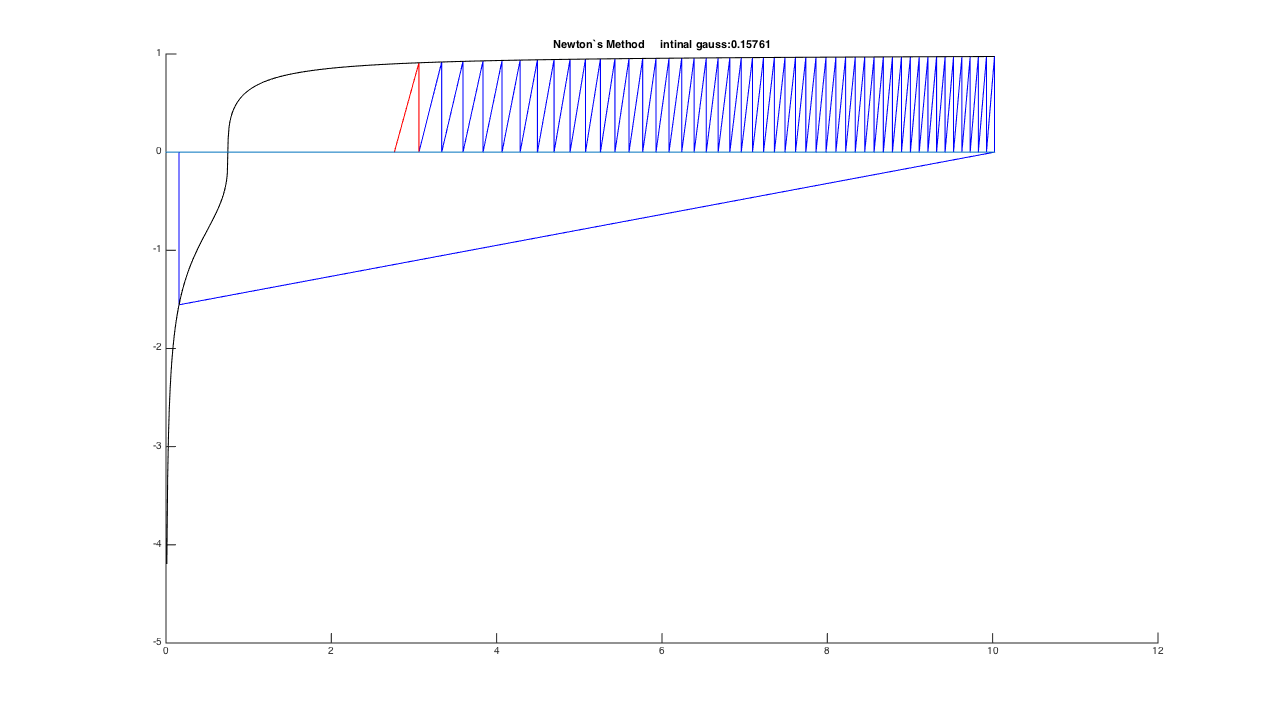
\includegraphics[scale=0.35]{plot1(2-4371).png} \]
		\[ 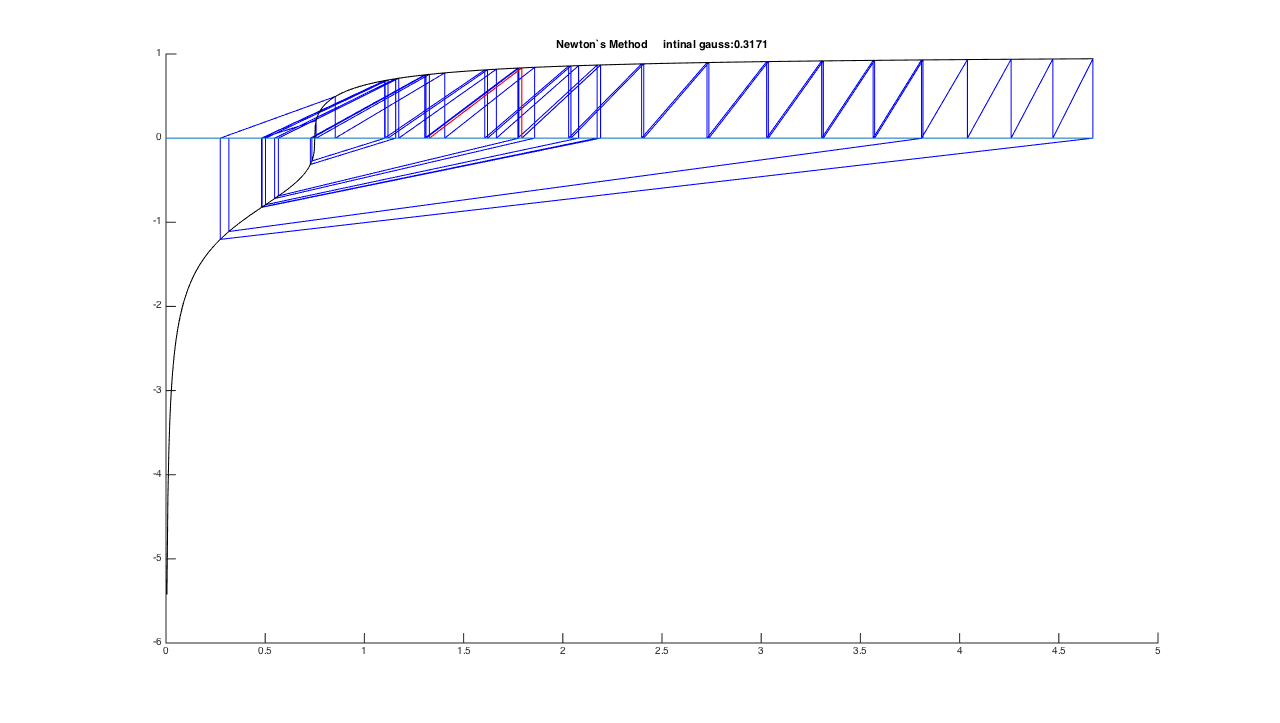
\includegraphics[scale=0.35]{plot(1-3285).png} \]
		\[ 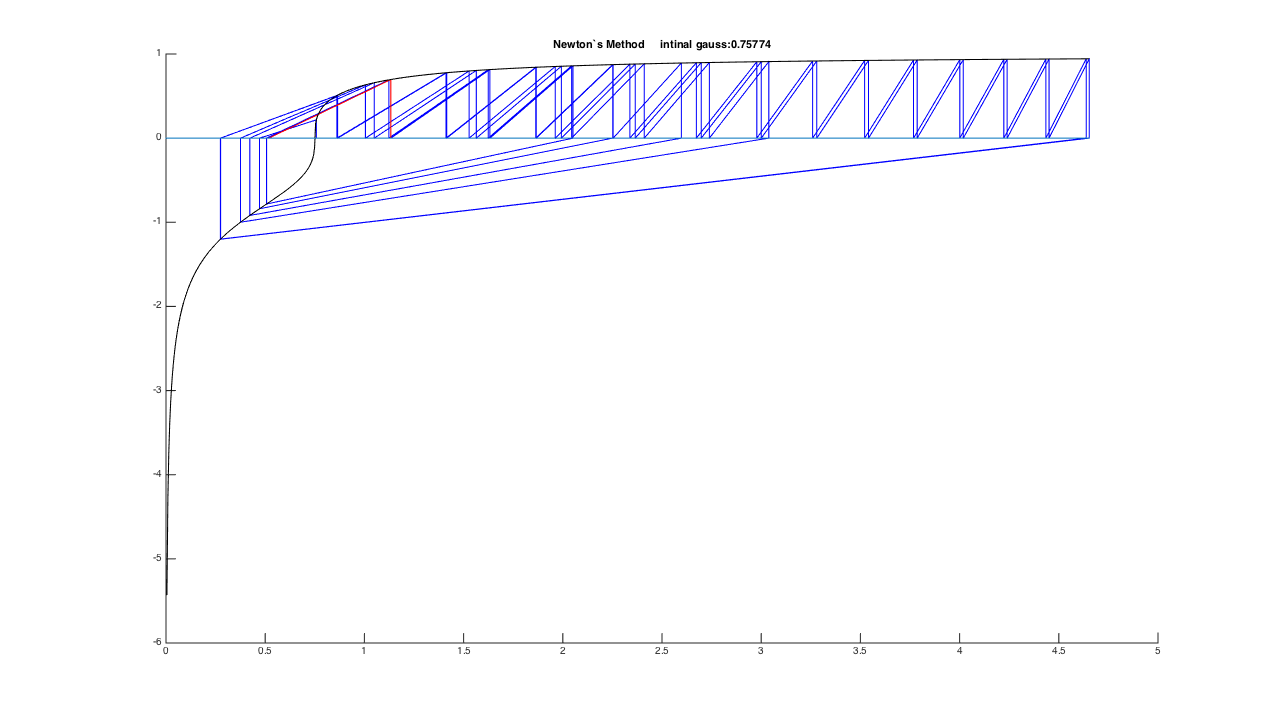
\includegraphics[scale=0.35]{plot(0-5184).png} \]
		\[ 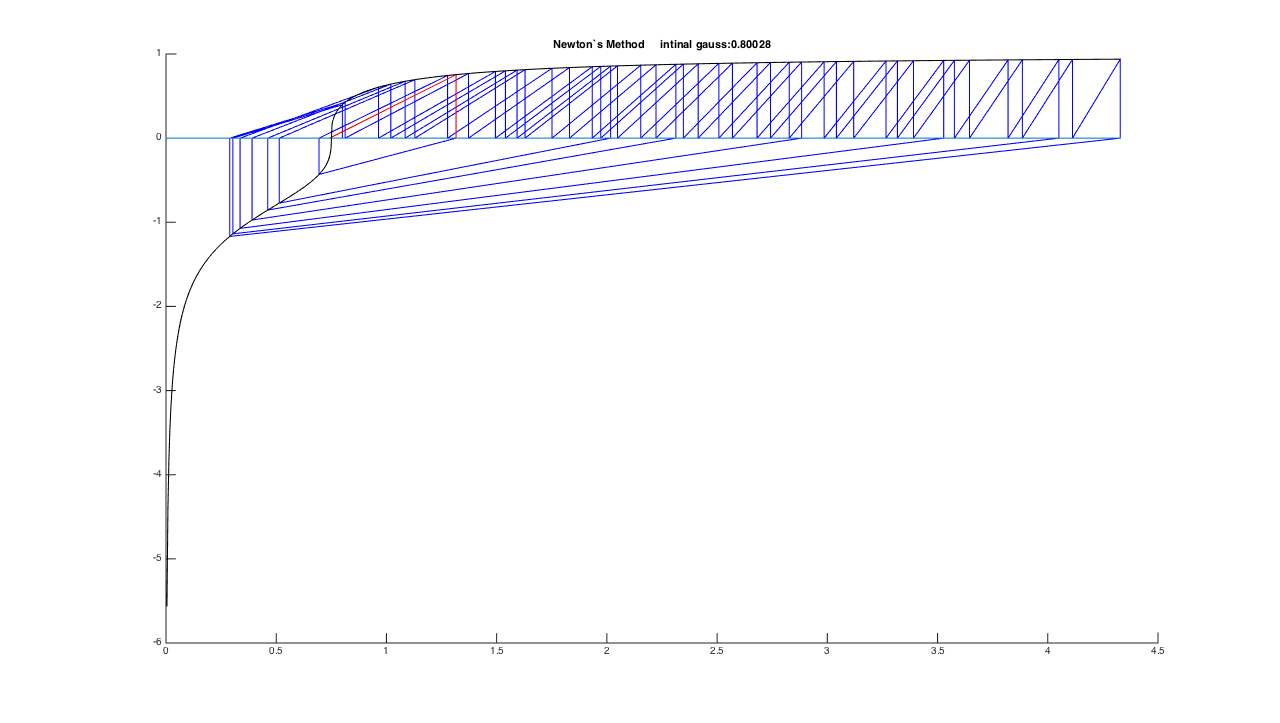
\includegraphics[scale=0.35]{plot2(0-7422).png} \]
	% part c
	\item From the plots, we could observe,
		\begin{itemize}
		\item Base on different initial guess with fixed iteration the $Newton's \ method$ might converge or diverge.
		\item For a $Newton's \ method$ with some initial guess, the function may converge for some certain iterations (i.e it may first converge then diverge). 
		\end{itemize}
	\end{enumerate}
	
\end{enumerate}

\end{document}